\documentclass[12pt,a4paper]{article}

% --- Encoding & Fonts ---
\usepackage[T1]{fontenc}
\usepackage[utf8]{inputenc}
\usepackage{lmodern}
\usepackage{microtype}

% --- Page Geometry ---
\usepackage[top=2.5cm, bottom=2.5cm, left=2.5cm, right=2.5cm]{geometry}

% --- Language ---
\usepackage[english]{babel}

% --- Math (required for \text{} inside $...$) ---
\usepackage{amsmath}

% --- Tables & Figures ---
\usepackage{booktabs}
\usepackage{tabularx}
\usepackage{graphicx}
\usepackage{float}
\usepackage{caption}
\captionsetup{font=small, labelfont=bf}

% --- Color (must precede listings) ---
\usepackage{xcolor}

% --- Code Listings ---
\usepackage{listings}
\lstset{
  basicstyle=\ttfamily\footnotesize,
  backgroundcolor=\color{gray!10},
  frame=single,
  breaklines=true,
  breakatwhitespace=false,
  captionpos=b,
  numbers=left,
  numberstyle=\tiny\color{gray},
  xleftmargin=2em,
  framexleftmargin=1.5em,
  showstringspaces=false,
}

% --- Spacing ---
\usepackage{setspace}
\setstretch{1.3}

% --- Section Formatting ---
\usepackage{titlesec}
\titleformat{\section}{\large\bfseries}{\thesection}{1em}{}
\titleformat{\subsection}{\normalsize\bfseries}{\thesubsection}{1em}{}
\titlespacing*{\section}{0pt}{1.5ex plus .5ex minus .2ex}{0.8ex plus .2ex}
\titlespacing*{\subsection}{0pt}{1.2ex plus .3ex minus .2ex}{0.5ex plus .1ex}

% --- Monospace-wrapping column type for tabularx ---
\newcolumntype{M}{>{\ttfamily\footnotesize\raggedright\arraybackslash}X}

% --- Hyperlinks (always load last) ---
\PassOptionsToPackage{hyphens}{url}
\usepackage[hidelinks, pdfauthor={Aditya Vikram},
  pdftitle={Open Data Integration with Accidents in Germany},
  pdfsubject={Web Engineering Term Paper}]{hyperref}

% ============================================================
\begin{document}

% --- Cover Page ---
\begin{titlepage}
\centering

\vspace*{1cm}

{\LARGE\bfseries Technische Universit\"at Chemnitz}\\[0.5cm]
{\large Faculty of Computer Science}

\vspace{1.5cm}

\rule{\textwidth}{0.4pt}\\[0.5cm]
{\LARGE\bfseries Open Data Integration with Accidents in Germany}\\[0.4cm]
{\large A Reproducible Spatio-Temporal Data Platform}\\[0.3cm]
\textit{--- DWT\_Project ---}\\[0.2cm]
\rule{\textwidth}{0.4pt}

\vspace{1.5cm}

\begin{tabular}{rl}
  \textbf{Subject:}            & Datenbanken und Webtechniken \\[4pt]
  \textbf{Course:}             & Web Engineering \\[4pt]
  \textbf{Author:}             & Aditya Vikram \\[4pt]
  \textbf{Study Course:}       & Web Engineering \\[4pt]
  \textbf{Matriculation No.:}  & 910541 \\[4pt]
  \textbf{Submission Date:}    & 25.06.2026 \\
\end{tabular}

\vfill
{\small Technische Universit\"at Chemnitz, 09107 Chemnitz, Germany}
\end{titlepage}

% --- Table of Contents ---
\tableofcontents
\newpage

% ============================================================
\section{Introduction and Data Sources}

German traffic-safety statistics are fragmented across at least four authoritative sources --- Destatis Unfallatlas, BKG Regionalatlas, GENESIS/Regionalstatistik, and GV-ISys --- each published in different formats, character encodings, and administrative-region vintages. AGS codes shift with every territorial reorganisation, making cross-source joins error-prone. DWT\_Project consolidates these sources into a single canonical schema exposed through a documented REST API and an interactive web frontend.

The platform achieves six concrete goals: a unified relational schema with PostGIS spatial extensions; a fully auto-generated OpenAPI~3.1 specification; a lightweight browser-based map frontend requiring no build step; a mandatory one-command update script (\texttt{python -m etl.update}); complete provenance for every row via import run audit records; and a one-command Docker Compose stack for reproducing the full environment on any machine.

Four open datasets feed the system, summarised in Table~\ref{tab:sources}.

\begin{table}[H]
\centering
\caption{Data sources}
\label{tab:sources}
\begin{tabularx}{\textwidth}{lXll}
\toprule
\textbf{Source} & \textbf{Content} & \textbf{Format} & \textbf{License} \\
\midrule
Destatis Unfallatlas      & $\approx$3\,M personal-injury accidents, 2016--2024 & CSV (Latin-1, \texttt{;}) & dl-de/by-2-0 \\
BKG Regionalatlas         & Admin-region polygons (states, districts, municipalities) & Shapefile (EPSG:25832) & dl-de/by-2-0 \\
GENESIS/Regionalstatistik & Population and registered cars by region/year & CSV (UTF-8) & dl-de/by-2-0 \\
GV-ISys (Destatis)        & Canonical AGS code table and reorganisation history & CSV & dl-de/by-2-0 \\
\bottomrule
\end{tabularx}
\end{table}

% ============================================================
\section{Technologies Used and Motivation}

\begin{table}[H]
\centering
\caption{Technology stack}
\label{tab:stack}
\begin{tabularx}{\textwidth}{llX}
\toprule
\textbf{Layer} & \textbf{Choice} & \textbf{Motivation} \\
\midrule
Database  & PostgreSQL 16 + PostGIS 3.4   & Native KNN \texttt{<->} operator, GiST indexing; \texttt{ST\_DWithin} avoids app-side filtering on 3\,M rows \\
Backend   & Python 3.11 + FastAPI          & Auto-generated OpenAPI 3.1; async handlers; declarative 422 validation \\
ORM       & SQLAlchemy 2.0 + GeoAlchemy2   & Type-safe schema; raw-SQL \texttt{text()} escape for PostGIS operators \\
ETL       & pandas, httpx, pyshp, pyproj   & Vectorised 3\,M-row CSV processing; CRS reprojection for BKG shapefiles \\
Frontend  & Vanilla JS + Leaflet + Deck.GL & No build step; GPU-accelerated \texttt{HexagonLayer} \\
Infra     & Docker Compose + pytest        & One-command reproducibility; integration tests for all seven examiner queries \\
\bottomrule
\end{tabularx}
\end{table}

Three choices deserve explicit justification. PostGIS was chosen over plain PostgreSQL with application-side spatial filtering: a \texttt{ST\_DWithin} index scan on 3\,M rows runs in under 10\,ms; Python-side filtering takes seconds. FastAPI was chosen over Flask because it generates a fully conformant OpenAPI specification without plugins, fulfilling the rubric's API documentation requirement at zero extra cost. The frontend uses no build step so that an examiner can audit every line of JavaScript in the browser DevTools without installing Node.js.

% ============================================================
\section{Architecture and Workflow}

\subsection{System Architecture}

\begin{figure}[H]
\centering
\begin{lstlisting}[numbers=none]
+--------------------------------------------------+
|  Docker Compose                                  |
|                                                  |
|  +--------------------+   +-------------------+  |
|  | PostgreSQL 16      |<--| FastAPI (uvicorn)  |  |
|  | + PostGIS 3.4      |   | port 8000          |  |
|  +--------------------+   +--------+----------+  |
|           ^                        |              |
+-----------+------------------------+--------------+
            |  ETL sidecar           | StaticFiles /
            |  python -m etl.update  | frontend/
            |                        v
            |                   Browser
            |               (Leaflet + Deck.GL)
            |
  [Unfallatlas CSVs]  [BKG Shapefiles]
  [GENESIS CSVs]      [GV-ISys CSV]
\end{lstlisting}
\caption{System architecture. ETL runs as a sidecar; FastAPI serves REST API and static frontend on port~8000.}
\label{fig:arch}
\end{figure}

Data flows in one direction: the ETL downloads source files, validates and transforms each row, and writes to PostgreSQL with \texttt{ON CONFLICT} idempotency. FastAPI reads from PostgreSQL and exposes results as JSON. The static frontend fetches from FastAPI endpoints and renders with Leaflet and Deck.GL.

\subsection{Source Selection and Access Paths}

Each source was chosen for a specific combination of content and format. \textbf{Unfallatlas} yearly CSVs were preferred over the WFS feed because the WFS lacks per-year participant-flag columns (\texttt{IstRad}, \texttt{IstFuss}, etc.) needed for examiner questions 5--7. Files are Latin-1 encoded with \texttt{;} separators. \textbf{BKG Regionalatlas} shapefiles are reprojected from EPSG:25832 to EPSG:4326 for storage; the metric copy is retained in \texttt{cell\_geom\_proj} for KNN queries. \textbf{GENESIS} population and car tables use a fixed URL pattern; the separator is detected at runtime. \textbf{GV-ISys} supplies the canonical AGS code list and the reorganisation table mapping historical codes to current 2024 AGS.

Every ingestion creates one row in \texttt{import\_runs} recording source name, URL, SHA-256 of the downloaded file, retrieval timestamp, status, rows inserted, and rows updated. Every fact row references \texttt{import\_run\_id}, enabling exact audit trails.

\subsection{Schema Mapping, Harmonisation and Indexing}

\begin{figure}[H]
\centering
\begin{lstlisting}[numbers=none]
sources <-- import_runs --> (all fact tables carry import_run_id)
                |
                v
            regions <---- indicator_values <-- indicators
                |
                +---> accidents
                +---> accident_zones
                +---> regions_history (old_ags -> new_ags)
                         lookup_codes
\end{lstlisting}
\caption{Nine-table schema. Fact tables join to \texttt{regions} via AGS; every fact row carries \texttt{import\_run\_id}. Full DDL: \texttt{db/init/01\_schema.sql}.}
\label{fig:schema}
\end{figure}

\textbf{AGS as universal join key.} \texttt{regions.ags} is declared \texttt{TEXT PRIMARY KEY} throughout --- never \texttt{INTEGER} --- because leading zeros are semantically significant (e.g.\ Saxony = \texttt{"14"}). Historical codes are resolved via \texttt{regions\_history(old\_ags, new\_ags, change\_date)} before insertion.

\textbf{Long-format indicators.} Population and car-registration figures are stored in \texttt{indicator\_values(indicator\_id, region\_id, year, value)} rather than as wide columns. This allows new indicators without schema migration and enables year-over-year queries with a single index scan.

\textbf{Indexes.} GiST indexes on \texttt{accidents.geom} and \texttt{accident\_zones.cell\_geom\_proj} support spatial range queries and KNN. B-tree indexes on \texttt{(year)}, \texttt{(region\_id, year)}, and \texttt{(year, category)} accelerate all aggregate endpoints. A partial index on \texttt{(region\_id, year) WHERE category = 1} serves fatal-rate ranking (fatal $\approx$ 2.5\,\% of rows).

\textbf{Dual-SRID design.} API-facing geometries are stored in EPSG:4326 for JSON portability. Hotspot grid cells additionally carry \texttt{cell\_geom\_proj GEOMETRY(POLYGON, 25832)}, a precomputed metric copy for sub-millisecond KNN via PostGIS \texttt{<->}. Computing CRS transforms on 3\,M rows at query time is prohibitively slow; the precomputed column eliminates that cost.

\subsection{API Design Decisions}

Every response follows a standard envelope:

\begin{lstlisting}[language={},caption={Standard API response envelope}]
{
  "results": [ { "...": "..." } ],
  "metadata": {
    "total_count": 1234,
    "sources_used": ["unfallatlas"],
    "license": "dl-de/by-2-0",
    "license_url": "https://www.govdata.de/dl-de/by-2-0",
    "import_run_id": 12,
    "retrieved_at": "2026-06-25T18:00:00Z"
  }
}
\end{lstlisting}

The envelope ensures license attribution reaches every consumer without separate documentation. The API exposes 15 endpoints grouped by purpose: \texttt{regions}, \texttt{accidents}, \texttt{aggregates}, \texttt{zones}, \texttt{metadata}, and \texttt{healthz} (full reference in Appendix~\ref{app:api}).

Error semantics follow a strict convention: HTTP~422 for any unknown or out-of-range enum. The API never performs a silent full-scan on an unrecognised filter value.

\subsection{Update Workflow and Reproducibility}

\texttt{python -m etl.update} runs five sequential phases: (1)~sources, (2)~regions, (3)~accidents, (4)~indicators, (5)~zones. Each phase is independently invocable via \texttt{--source}, and \texttt{--dry-run} validates download and parsing without writing to the database.

Every insert uses \texttt{ON CONFLICT DO NOTHING} or \texttt{ON CONFLICT DO UPDATE} on the natural key, making all phases idempotent. \texttt{docker compose up -d} starts the full stack within 60~seconds. Per-indicator failure isolation means one malformed GENESIS file does not abort the population phase.

% ============================================================
\section{Challenges}

\subsection{Silent State-Code Drops}

\textbf{Problem.} The \texttt{/accidents} endpoint accepted a \texttt{state} query parameter. An unrecognised code (e.g.\ \texttt{SX} instead of \texttt{SN}) returned HTTP~200 with an empty result set. A user seeing zero results assumed the data was absent.

\textbf{Mitigation.} All string-enum parameters are validated against a closed allowlist using FastAPI's \texttt{Query(enum=[...])}. Unrecognised values return HTTP~422 with a structured error naming the offending parameter and listing valid values.

\textbf{Lesson.} Returning 200 for an unmatched filter is a silent-failure anti-pattern. APIs must reject invalid inputs explicitly.

\subsection{NaN-to-False in Participant Flags}

\textbf{Problem.} Unfallatlas CSVs encode absent participant flags as empty cells, which pandas reads as \texttt{NaN}. Writing such a column to PostgreSQL via SQLAlchemy silently coerced \texttt{NaN} to \texttt{False}, so ``not recorded'' became ``not involved'' --- corrupting bicycle and pedestrian counts used in examiner questions 5 and~6.

\textbf{Mitigation.} All participant-flag columns are explicitly mapped through \texttt{pd.NA} $\rightarrow$ \texttt{SQL NULL} before insertion. The ETL includes a post-insert assertion: the count of \texttt{NULL} flags must be non-zero for any year before 2018, where blanks are structurally expected.

\textbf{Lesson.} Cross-language type coercions between Python \texttt{NaN}, \texttt{None}, and SQL \texttt{NULL} are invisible until they corrupt query results.

\subsection{The AGS Leading-Zero Problem}

\textbf{Problem.} AGS codes for eastern German states begin with \texttt{0} (e.g.\ \texttt{"014"}). A join column typed as \texttt{INTEGER} silently strips the leading zero, making \texttt{"014"} equal to~14. Cross-source joins returned zero matches for six affected states.

\textbf{Mitigation.} \texttt{regions.ags} is declared \texttt{TEXT PRIMARY KEY} throughout. The ETL validates that AGS values contain only digit strings of length~2, 5, or~8 before insertion.

\textbf{Lesson.} Identifiers carrying semantic structure in leading zeros must be stored as strings at the schema level.

% ============================================================
\section{Limitations, Plausibility Checks and Data Quality}

\subsection{Plausibility Checks Performed During ETL}

The ETL enforces the following validation gates before any row reaches the database:

\begin{itemize}
  \item \textbf{Spatial bounds.} $(lat, lon)$ must fall within Germany's bounding box
        ($47.27$--$55.06^\circ$N, $5.87$--$15.04^\circ$E). Out-of-bounds rows are logged and rejected.
  \item \textbf{Temporal bounds.} $\text{year} \in [2016, 2024]$; $\text{month} \in [1, 12]$;
        $\text{hour} \in [0, 23]$; $\text{day\_of\_week} \in [1, 7]$.
  \item \textbf{Categorical bounds.} $\text{category} \in \{1, 2, 3\}$; participant flags
        $\in \{\text{TRUE}, \text{FALSE}, \text{NULL}\}$ (\texttt{NaN} $\rightarrow$ \texttt{NULL}).
  \item \textbf{Referential integrity.} Every \texttt{region\_id} must resolve to a known AGS
        in \texttt{regions} directly or via \texttt{regions\_history}.
  \item \textbf{Indicator sanity.} Population $> 0$; cars-per-1000-population $\in [1, 2000]$.
  \item \textbf{Row-count gate.} Import aborts if the file yields $<$50\,\% of the prior year's row count.
\end{itemize}

\subsection{Known Data Quality Issues}

\textbf{AGS reorganisation gaps.} \texttt{regions\_history} covers documented mergers up to 2024 per GV-ISys, but some micro-renames are unpublished. Pre-2018 accidents in reorganised districts may attach to a parent-level AGS.

\textbf{Indicator coverage gaps.} GENESIS publishes population at municipality level but registered-car counts only at district level. Municipality-level fatal-rate queries use district-level denominators; this is documented in every rate response's \texttt{metadata} block.

\textbf{2016--2017 surrogate UIDs.} The \texttt{UIDENTSTLAE} identifier was introduced in 2018. Earlier rows use a SHA-1 surrogate from \texttt{(year, month, day\_of\_week, hour, lat, lon)}.

\textbf{Geocoding precision.} Unfallatlas coordinates are rounded to a $\approx$50\,m privacy-preserving grid. KNN distances below this threshold are not street-level precise.

\textbf{License obligation.} dl-de/by-2-0 requires attribution. DWT\_Project propagates license and URL through every API response envelope.

\subsection{Limitations of Scope}

Four sources satisfy the rubric's $\geq 3$ requirement; hospital admission records, real-time vehicle telemetry, and weather data are out of scope. Data freshness is limited by Unfallatlas's 9--12 month publication lag; the 2025 accident year is not yet available at submission. The \texttt{/healthz/data-quality} endpoint reports row counts and the most recent import timestamp; deeper anomaly detection is deferred. All SQL is parameterised; the two exceptions --- column-name interpolation and sort-axis selection --- are protected by closed allowlists with \texttt{assert} guards.

% ============================================================
\newpage
\begin{thebibliography}{99}

\bibitem{destatis-license}
Destatis, ``dl-de/by-2-0 Datenlizenz Deutschland,''
\url{https://www.govdata.de/dl-de/by-2-0}.

\bibitem{postgis}
PostGIS Development Group, \textit{PostGIS 3.4 Documentation},
\url{https://postgis.net/docs/}.

\bibitem{fastapi}
S.~Ramirez, ``FastAPI,'' \url{https://fastapi.tiangolo.com/}.

\bibitem{sqlalchemy}
SQLAlchemy Authors, \textit{SQLAlchemy 2.0 Documentation},
\url{https://docs.sqlalchemy.org/}.

\bibitem{geoalchemy}
E.~Lemoine, ``GeoAlchemy 2,'' \url{https://geoalchemy-2.readthedocs.io/}.

\bibitem{leaflet}
Leaflet Contributors, ``Leaflet,'' \url{https://leafletjs.com/}.

\bibitem{deckgl}
Deck.GL Authors, ``Deck.GL,'' \url{https://deck.gl/}.

\bibitem{unfallatlas}
Destatis, ``Unfallatlas,'' \url{https://unfallatlas.statistikportal.de/}.

\bibitem{bkg}
BKG, ``Regionalatlas Deutschland,'' \url{https://gdz.bkg.bund.de/}.

\bibitem{genesis}
Destatis, ``Regionalstatistik / GENESIS-Online,''
\url{https://www.regionalstatistik.de/}.

\bibitem{gvisys}
Destatis, ``GV-ISys --- Gemeindeverzeichnis,''
\url{https://www.destatis.de/DE/Themen/Laender-Regionen/Regionales/Gemeindeverzeichnis/}.

\bibitem{epsg}
EPSG.io, ``Coordinate Systems Worldwide,'' \url{https://epsg.io/}.

\end{thebibliography}

% ============================================================
\newpage
\appendix
\section{API Documentation}
\label{app:api}

\subsection*{Access}

\begin{itemize}
  \item \textbf{Swagger UI (interactive):} \url{http://localhost:8000/docs}
  \item \textbf{Raw OpenAPI 3.1 JSON:} \url{http://localhost:8000/openapi.json}
  \item \textbf{Exported snapshot:} \texttt{api-docs/openapi.json} (committed to repository)
\end{itemize}

No authentication required. Every response carries \texttt{metadata.license = "dl-de/by-2-0"} and \texttt{metadata.license\_url}.

\subsection*{Endpoint Reference}

\begin{table}[H]
\centering
\caption{API endpoint reference}
\label{tab:endpoints}
\begin{tabularx}{\textwidth}{llXl}
\toprule
\textbf{Method} & \textbf{Path} & \textbf{Purpose} & \textbf{Codes} \\
\midrule
GET & \texttt{/regions}                       & List regions                    & 200, 422 \\
GET & \texttt{/regions/\{ags\}}               & Single region                   & 200, 404 \\
GET & \texttt{/accidents}                     & Accident records (bbox filter)  & 200, 422 \\
GET & \texttt{/aggregates/accidents}          & Count by region/year            & 200, 422 \\
GET & \texttt{/aggregates/accident-rate}      & Rate per 100k pop or cars       & 200, 422 \\
GET & \texttt{/aggregates/accident-rate/top}  & Top districts by rate           & 200, 422 \\
GET & \texttt{/zones/nearest}                 & Nearest hotspot cell            & 200, 422 \\
GET & \texttt{/zones/around}                  & Cells in radius                 & 200, 422 \\
GET & \texttt{/zones/nearby-hazards}          & Top~5 hotspots $\leq$500\,m    & 200, 422 \\
GET & \texttt{/metadata/sources}              & Dataset registry                & 200      \\
GET & \texttt{/metadata/import-runs}          & ETL audit log                   & 200      \\
GET & \texttt{/healthz}                       & API liveness                    & 200      \\
GET & \texttt{/healthz/data-quality}          & Row counts + last import        & 200      \\
\bottomrule
\end{tabularx}
\end{table}

All coordinate parameters validate $\text{lat} \in [47.27,\,55.06]$ and $\text{lon} \in [5.87,\,15.04]$; out-of-range values return~422.

\subsection*{Examiner-Question Cookbook}

\begin{table}[H]
\centering
\caption{Endpoints for the seven mandatory examiner queries}
\label{tab:cookbook}
\footnotesize
\begin{tabularx}{\textwidth}{clMl}
\toprule
\textbf{Q\#} & \textbf{Question} & \textbf{Endpoint} & \textbf{Check} \\
\midrule
Q1 & Earliest year national data?   & /aggregates/accidents?level=state                                                                          & Min year        \\
Q2 & Accidents Saxony 2023?          & /accidents?state=SN\&year=2023                                                                             & total\_count    \\
Q3 & Earliest year NRW?              & /aggregates/accidents?level=state\&state=NW                                                                & Min year        \\
Q4 & Earliest year MV?               & /aggregates/accidents?level=state\&state=MV                                                                & Min year        \\
Q5 & Pedestrians Berlin 2023?        & /accidents?state=BE\&year=2023\&participant=pedestrian                                                     & total\_count    \\
Q6 & Top districts cars rate?        & /aggregates/accident-rate/top?denominator=cars\_pkw\&year=2023                                             & results[0..4]   \\
Q7 & Top~5 fatal rate per 100k?      & /aggregates/accident-rate/top?severity=fatal\&denominator=population\&min\_population=50000\&limit=5       & results[0..4]   \\
\bottomrule
\end{tabularx}
\end{table}

\begin{figure}[H]
\centering
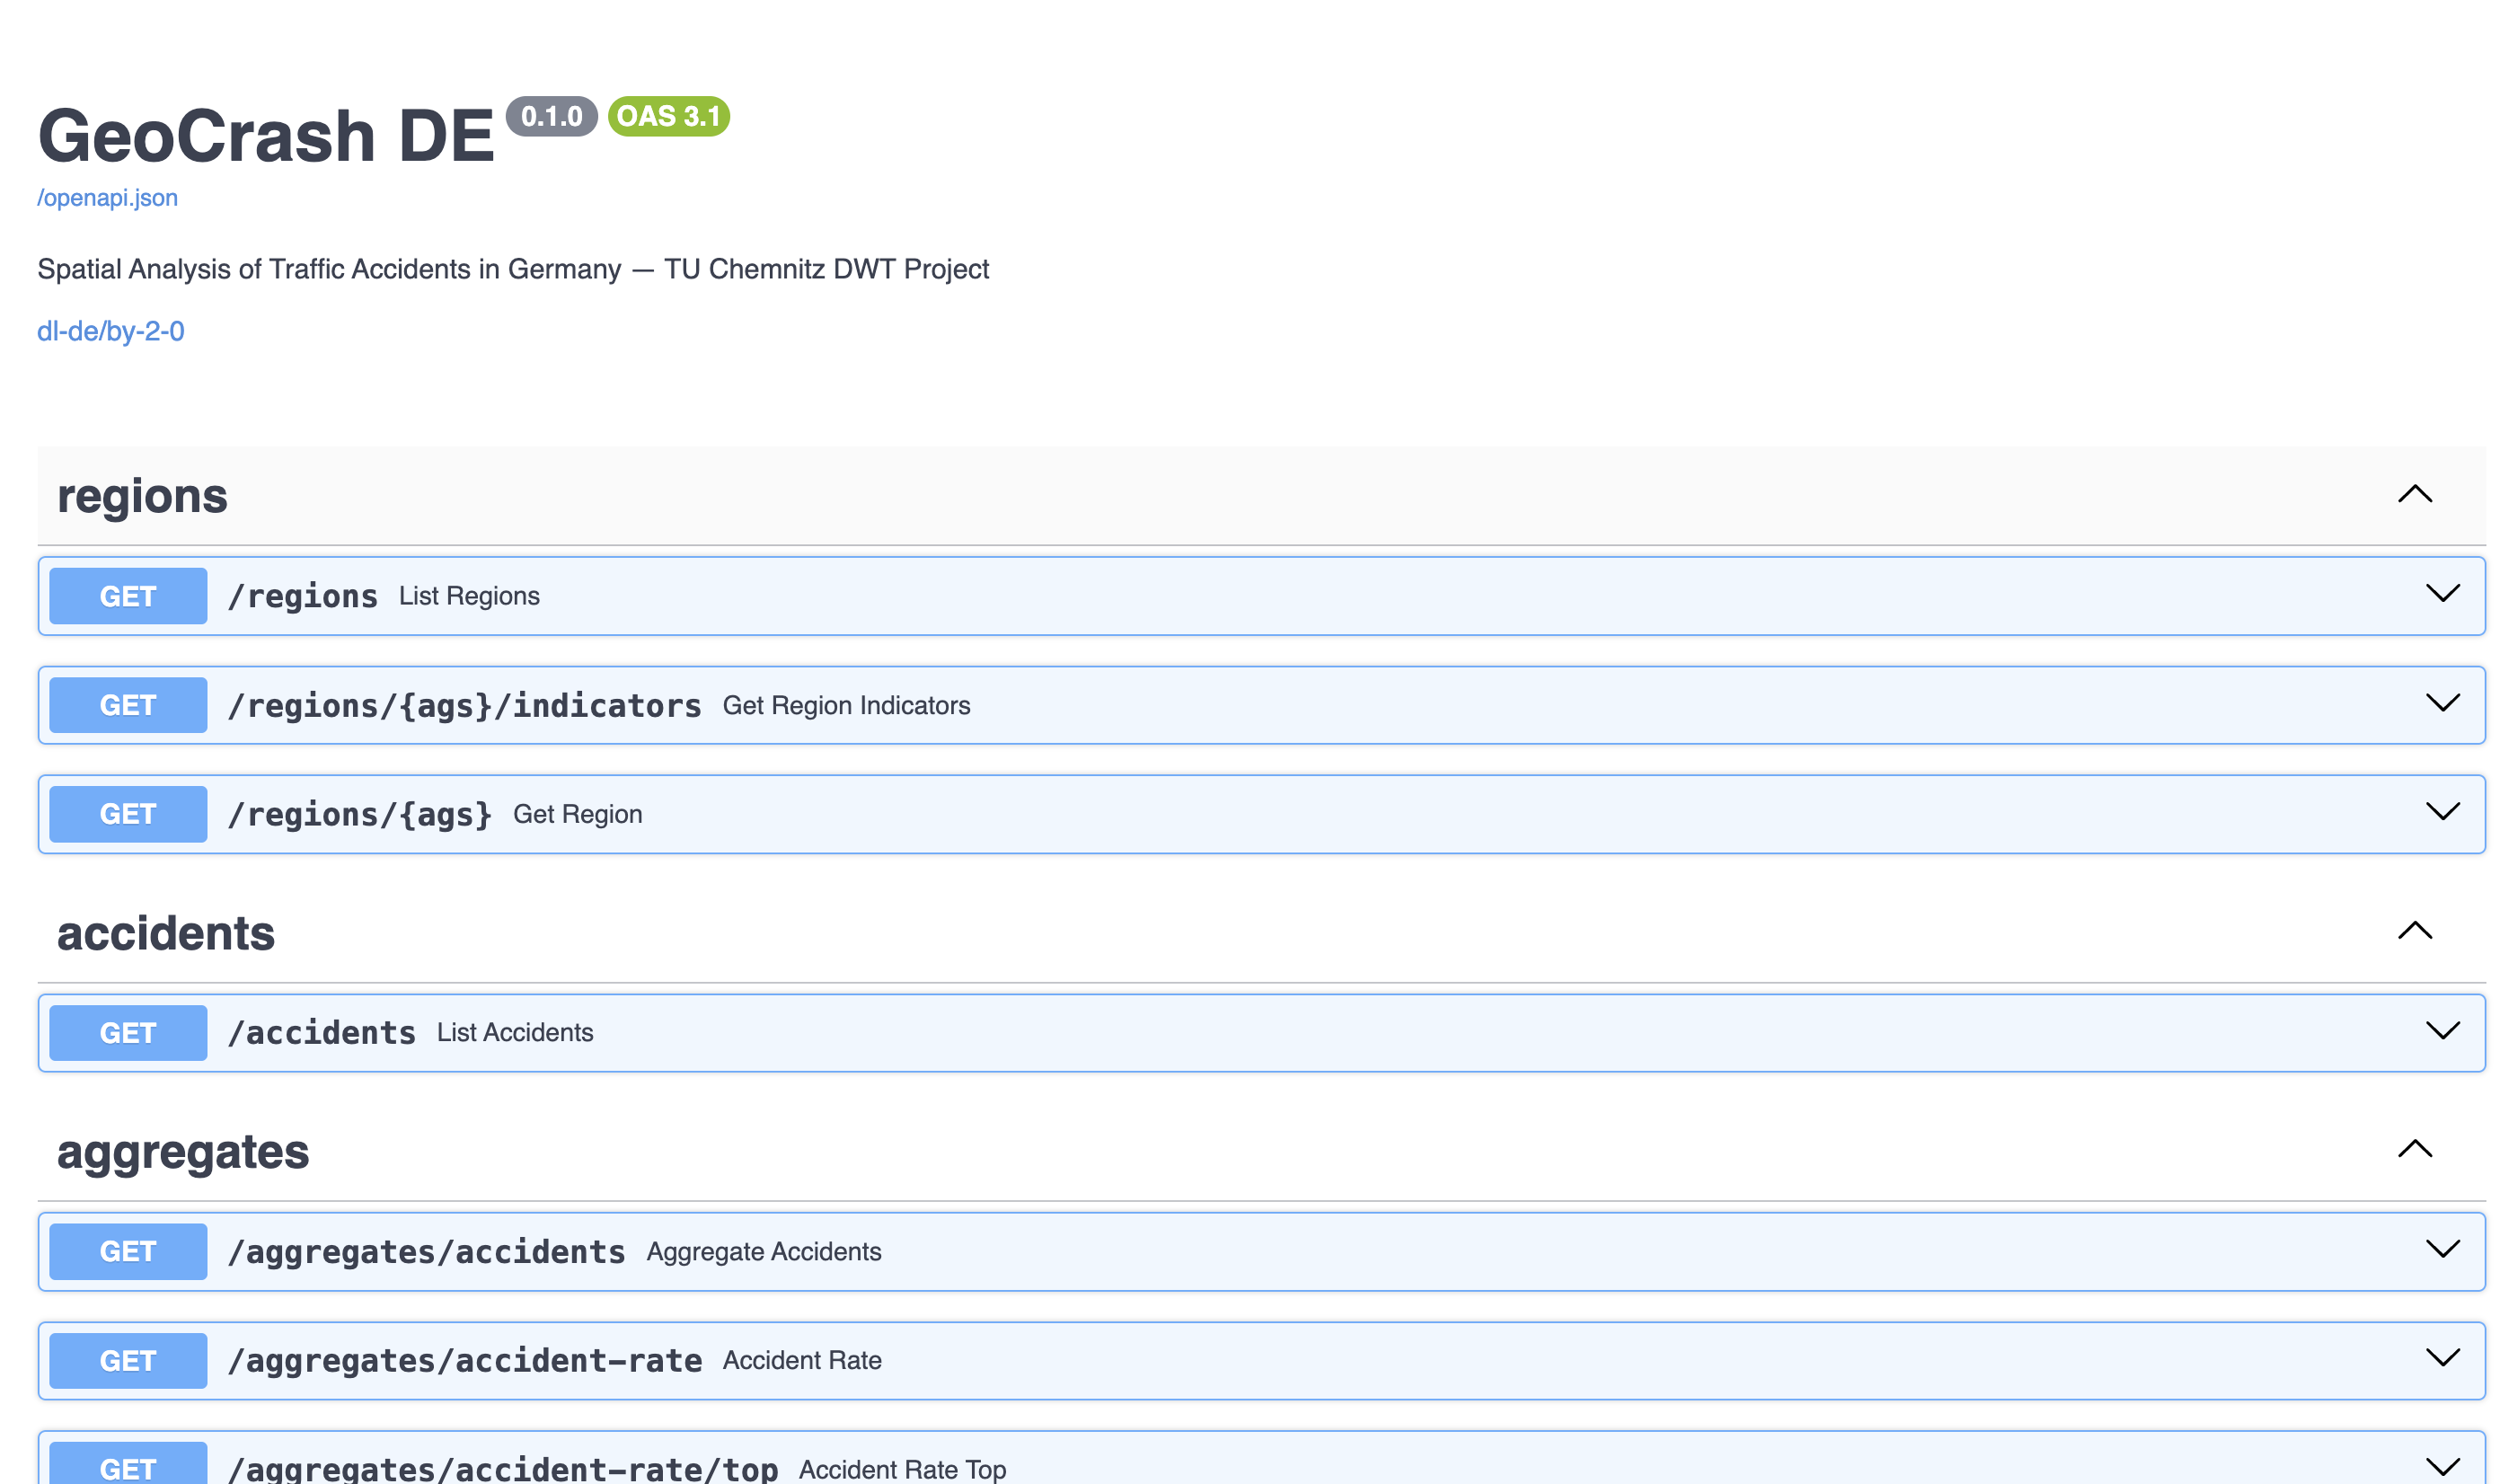
\includegraphics[width=\textwidth]{swagger-ui.png}
\caption{Swagger UI --- GeoCrash DE API endpoint list at \texttt{http://localhost:8000/docs}.}
\label{fig:swagger}
\end{figure}

\end{document}
